
\subsection*{Les politiques documentaires en bibliothèques, définition et enjeux d'un outil stratégique}

\begin{quotation}
		Faire de la politique documentaire, c'est faire vivre un établissement à travers toutes ses facettes\footnote{Depuydt (Yaëlle), « Faire de la politique documentaire, c’est faire vivre un établissement à travers toutes ses facettes » : entretien avec Yaëlle Depuydt », Bulletin des bibliothèques de France (BBF), 2022-1. \url{https://bbf.enssib.fr/consulter/bbf-2022-00-0000-004}}.
\end{quotation}
C'est ainsi que Yaëlle Depuydt, alors directrice du projet de médiathèque hybride et participative de Cysoing, introduisait la politique documentaire dans un entretien accordé au Bulletin des bibliothèques de France (BBF) en 2022. 

A l'instar des archives, guidées par les \enquote{4 C} (collecter, classer, conserver, communiquer), les bibliothèques sont aussi guidées par trois maîtres-mots qui représentent leurs missions fondamentales  : l'acquisition, la conservation et l'accessibilité dont la politique documentaire régit l'organisation et l'articulation.

Selon la traditionnelle définition de Bertrand Calenge, 
\begin{quotation}
	La politique documentaire recouvre au sein d'une bibliothèque l'ensemble des processus visant à contrôler le développement des collections. Elle recouvre la politique d'acquisition, la politique de conservation (incluant le désherbage), la politique d'accessibilité (incluant les modalités d'organisation et de communication des collections).\footnote{Calenge (Bertrand), \textit{Bibliothèques et politiques documentaires à l'heure d'Internet}, Paris, Éditions du Cercle de la Librairie, 2008 ; 264 p. (ISBN 978-2-7654-0962-5).}
\end{quotation}

La politique documentaire, si elle s'intéresse séparément à toutes les facettes des bibliothèques, a également le rôle d'articuler ces facettes, impliquant ainsi \enquote{un management et une stratégie de l'établissement}\footnote{Henard (Charlotte), \textit{La politique documentaire, de quoi parle-t-on et comment faire ?}, support de cours de l'ABF, Toulouse, Médiad'Oc, 2024-2025.}. Cette stratégie prend aussi en compte les aspects budgétaires et partenariaux.

La politique documentaire est donc une réflexion collective mobilisant toute une équipe autour d'un projet de gestion des collections, de leur acquisition à leur médiation, sous la coupe d'une tutelle politique et fonctionnelle en lien avec la direction de la bibliothèque. 
Elle devient donc un enjeu managérial, financier et juridique dépassant même les horizons de la bibliothèque. En effet, dans la configuration actuelle de travail en réseau où il existe des groupes de médiathèques et d'universités, la politique documentaire n'y est donc pas pensée par établissement mais à l'échelle du groupe. Le travail en réseau, fondamental en bibliothèque, s'il rend le processus de politique documentaire plus exigeant, permet en retour de produire des analyses plus fines du territoire afin de mieux cibler les attentes des usagers. 
Dans son entretien au Bulletin des bibliothèques de France (BBF), Yaëlle Depuydt utilise l'exemple des prix littéraires pour souligner la pertinence de l'élaboration d'une politique documentaire en réseau\footnote{Depuydt (Yaëlle), « Faire de la politique documentaire, c’est faire vivre un établissement à travers toutes ses facettes » : entretien avec Yaëlle Depuydt », Bulletin des bibliothèques de France (BBF), 2022-1. \url{https://bbf.enssib.fr/consulter/bbf-2022-00-0000-004}}. Une telle organisation permet en effet à un groupement de médiathèques de se répartir les achats de livres primés et ainsi d'éviter d'occuper une place précieuse en bibliothèque avec des livres qui seront empruntés seulement dans les six mois suivant l'attribution de leur prix. 
Par ailleurs, le travail en réseau permet également d'adopter une politique de communication commune, harmonisant les pratiques de valorisation des collections et facilitant l'expérience des usagers. 

Pour parvenir à une définition aussi complète que possible, il est nécessaire que la philosophie d'élaboration d'une politique documentaire diffère entre des bibliothèques de lecture publique et des bibliothèques universitaires. 

En bibliothèque de lecture publique, il est important de souligner l'aspect politique de la gestion documentaire, qui est avant tout un enjeu de politique publique défini par la hiérarchie. Ainsi, l'orientation de la politique documentaire est le fruit d'une concertation avec les élus, qu'ils soient spécialistes ou non. 
Thierry Giappiconi, ancien directeur de la bibliothèque municipale de Fresnes et membre du groupe Poldoc de l'ENSSIB, définissait ainsi la politique documentaire en bibliothèque de lecture publique : 
\begin{quotation}
	Une politique documentaire est l'expression formalisée et cohérente qu'une bibliothèque de service public donne de ses choix et priorités en matière de développement et de gestion des collections adaptées aux missions de la bibliothèque et conforme aux orientations et enjeux de politique publique de collectivé.
\end{quotation}

En bibliothèque universitaire, les missions traditionnelles des bibliothèques se doublent d'une mise à disposition des ressources pour les étudiants concernant la maîtrise de l'information documentaire. Dans un contexte de profonde mutation de l'information scientifique et technique (IST)\footnote{L’information scientifique et technique (IST) est l’ensemble des informations nécessaires aux professionnels de la recherche, de l'enseignement, de l'industrie et de l'économie, quelle que soit la discipline concernée. (Dictionnaire de l'ENSSIB) }, le secteur documentaire devient multiscalaire et le travail en réseau des bibliothèques universitaires se situe, en effet, non au niveau de la conservation d'une\enquote{bibliothèque-trésor\footnote{Pieyre (Clément), \textit{Les mutations de la politique documentaire dans l'enseignement supérieur et la recherche} :  entretien avec Clément Pierre, Bulletin des bibliothèques de France (BBF), 2022-1}}, comme peuvent parfois être perçues les missions des bibliothèques,  mais plutôt au niveau des conditions réunies pour permettre aux étudiants de maîtriser l'information, dans la continuité des formations d'EMI (Education aux médias et à l'information) dans le secondaire. L'image du \enquote{conservatoire de trésors} réduisant les collections à un stock laisse alors place à une vision où les collections correspondent au contraire à un flux documentaire.
\begin{quotation}
	Une définition extensive, utilisée particulièrement dans les universités, considère la politique documentaire comme l'ensemble des objectifs et processus pilotant la gestion de l'information, incluant non seulement les activités des bibliothèques, mais également la formation des étudiants à la maîtrise de l'information et les flux de ressources documentaires qui irriguent les composants de l'université.\footnote{Citation de Hervé le Crosnier, enseignant-chercheur à l’Université de Caen, lors d'un cours consacré à la culture numérique, disponible sur CanalU au format vidéo :  Qu’est-ce qu’un document ?, cette définition a été trouvée dans l'article de Catherine Muller : Muller (Catherine), \textit{Qu’est-ce qu’un document numérique au 21è siècle }? Exercice de repérages. DLIS. Consulté le 19 août 2026. \url {https://doi.org/10.58079/nt0s}}, cette définition est également reprise dans le dictionnaire de l'ENSSIB à l'entrée politique documentaire.
\end{quotation}

Ces définitions permettent de mettre en exergue les enjeux de la politique documentaire, instrument politique émanant d'un travail en réseau et impliquant tutelle et élus, direction et agents de la bibliothèque ainsi que ses usagers. Le premier enjeu de la politique documentaire, aussi appelée \enquote{Poldoc}, est donc éminemment politique. En effet, la politique documentaire doit faire l'objet d'un consensus entre les différentes parties prenantes, c'est-à-dire entre les groupes précédemment cités.

 Yaëlle Depuydt dans son entretien à la BBF\footnote{\textit{Ibid.}} expliquait que, pour réussir une politique documentaire, il fallait au minimum obtenir la validation de la tutelle et la validation des élus au moyen d'une communication transparente du projet. Elle conseille de mettre en place des outils, comme par exemple des ateliers ou des visites, pour y parvenir. 
Exercice de négociation et de pédagogie auprès des tutelles ou les élus qui ne sont pas toujours spécialistes, la politique documentaire nécessite un important investissement horaire de la direction et des agents de la bibliothèque. Si elle fédère l'équipe autour d'un projet commun, elle se doit également de rassembler les usagers autour du projet de la bibliothèque. 

La cohérence de la politique documentaire se situe également dans sa nécessaire synergie avec le territoire qui accueille la bibliothèque, ou, pour les bibliothèques spécialisées, avec le secteur dont elles sont spécialistes\footnote{Au sujet des bibliothèques spécialisées, nous aborderons, dans la prochaine sous-partie, le cas des bibliothèques musicales pour présenter les enjeux des politiques documentaires d'établissement spécialisés}.
Il est donc essentiel d'évaluer les besoins des usagers pour garantir la cohérence des collections et l'adéquation entre les besoins du public et l'offre proposée en bibliothèque. 
Pour assurer cette adéquation entre les besoins et l'offre de l'institution, les bibliothèques travaillent de plus en plus en réseau avec d'autres bibliothèques. Travailler collectivement sur un même projet au sein d'un groupement de bibliothèques permet d'affiner les besoins en se focalisant sur un territoire plus étendu et en mettant en place une offre élargie, où les collections d'une bibliothèque peuvent compléter les collections de la bibliothèque voisine.\\

Pour mener à bien ces projets collectifs, les autres enjeux cités par Yaëlle Depuydt sont le temps mais aussi la formation des agents - pour laquelle la CNFPT, l'ABF ou encore les centres de formation comme Médiadix, Médiad'oc ou Médial proposent de nombreuses conférences - et bien sûr les enjeux budgétaires. En outre, elle propose des outils pour aider à mettre en place une politique documentaire. Il s'agit de l'analyse du territoire, l'analyse des collections, les outils de cadrage de la politique documentaire (chartes des collections\footnote{Ce sera l'objet de la dernière sous-partie de ce chapitre \nameref{subsection:Un exemple de charte des collections, la charte des ressources de LaDocumenta.eu}}, plan de développement, fiches domaines...) et les outils d'évaluation.\\

Dès lors, il s'agit d'étudier comment se traduisent ces éléments théoriques  de définition dans le processus d'élaboration d'une politique documentaire. 
Comme nous l'avons vu, la politique documentaire englobe les missions majeures de la bibliothèque que sont la politique d'acquisition, la politique de conservation et la politique d'accessibilité. (Bertrand Calenge). 

\newpage
Dans un premier temps, la \textbf{politique d'acquisition} se conduit en douze étapes, soulignées par l'Association des bibliothécaires de France (ABF) en 1992. Ces douze étapes sont la traduction en actes des considérations théoriques de la politique documentaire. 

\begin{figure}[htbp]
	\centering
	% couleurs
	\definecolor{mainblue}{HTML}{1A365D}
	\definecolor{softbg}{HTML}{F7FAFC}
	\definecolor{bordergray}{HTML}{CBD5E0}
	\definecolor{textdark}{HTML}{2D3748}
	
	\begin{tikzpicture}[
		node distance=0.6cm and 0.5cm,
		block/.style={
			rectangle, 
			rounded corners=5pt, 
			draw=bordergray, 
			fill=softbg, 
			thick, 
			text width=4.5cm, 
			minimum height=1.4cm, 
			align=left, 
			font=\small\sffamily\color{textdark}
		},
		arrow/.style={
			->, 
			>=latex, 
			thick, 
			mainblue!70
		}
		]
		
		% Ajout du point après le numéro (#1.)
		\newcommand{\boxitem}[2]{%
			{\Large\bfseries\color{mainblue}#1.}\par\vspace{2pt}%
			#2%
		}
		
		% 2e ligne
		\node[block] (b1) {\boxitem{1}{Disposer d’un responsable de la politique documentaire}};
		\node[block, right=of b1] (b2) {\boxitem{2}{Mettre en commun les réflexions}};
		\node[block, right=of b2] (b3) {\boxitem{3}{Réfléchir aux publics}};
		
		% --- LIGNE 2 (4 à 6, de droite à gauche) ---
		\node[block, below=0.8cm of b3] (b4) {\boxitem{4}{Associer des partenaires à la réflexion}};
		\node[block, left=of b4] (b5) {\boxitem{5}{Évaluer les collections existantes}};
		\node[block, left=of b5] (b6) {\boxitem{6}{Établir des indicateurs de gestion des acquisitions}};
		
		% 3e ligne
		\node[block, below=0.8cm of b6] (b7) {\boxitem{7}{Formaliser les procédures de désherbage}};
		\node[block, right=of b7] (b8) {\boxitem{8}{Penser « réseaux »}};
		\node[block, right=of b8] (b9) {\boxitem{9}{Utiliser les répartitions budgétaires}};
		
		%4e ligne
		\node[block, below=0.8cm of b9] (b10) {\boxitem{10}{Choisir sans subir}};
		\node[block, left=of b10] (b11) {\boxitem{11}{Développer les compétences en acquisition}};
		\node[block, left=of b11] (b12) {\boxitem{12}{Produire un document de politique générale}};
		
		% ajout des flèches
		\draw[arrow] (b1) -- (b2);
		\draw[arrow] (b2) -- (b3);
		\draw[arrow] (b3.south) |- ([yshift=0.4cm]b3.south |- b4.north) -| (b4.north);
		
		\draw[arrow] (b4) -- (b5);
		\draw[arrow] (b5) -- (b6);
		\draw[arrow] (b6.south) |- ([yshift=0.4cm]b6.south |- b7.north) -| (b7.north);
		
		\draw[arrow] (b7) -- (b8);
		\draw[arrow] (b8) -- (b9);
		\draw[arrow] (b9.south) |- ([yshift=0.4cm]b9.south |- b10.north) -| (b10.north);
		
		\draw[arrow] (b10) -- (b11);
		\draw[arrow] (b11) -- (b12);
		
	\end{tikzpicture}
	\caption{Les 12 points de la politique d'acquisition (ABF, 1992)}
	\label{fig:politique-acquisition-abf-12points}
\end{figure}

Dans un second temps, la \textbf{politique de conservation}\footnote{Voir à ce sujet la fiche \enquote{politique de conservation} produite par la BnF, consultable à cette adresse : \url{https://www.bnf.fr/fr/politique-de-conservation}} regroupe les actions de conservation préventive des collections comme le contrôle des conditions hygrométriques des magasins, la reliure préventive, le dépoussiérage ainsi que le conditionnement des documents. La prévention repose également sur l'élaboration d'un plan d'urgence. Par ailleurs, la conservation curative s'entend comme la restauration de documents à des fins de limitations de dégradations. 
Aujourd'hui, ces traitements préventifs et curatifs s'enrichissent d'une préocuppation des collections numériques dans un souci de pérennité. C'est l'objet de l'outil SPAR (Système de Préservation et d'Archivage Réparti) dont s'est dotée la BnF en 2010. 
Toutefois, il ne faut pas oublier que la politique de conservation de la gestion documentaire concerne également les opérations de désherbage en bibliothèque. 
Le glossaire commun des Centres Régionaux de Formation aux Carrières des Bibliothèques (CRFCB) propose cette définition du désherbage, qui souligne bien la double dimension qu'il recouvre, et qui ne le réduit pas, comme trop souvent, à la seule élimination de documents. 
\begin{quotation}
	Le désherbage dans une bibliothèque se concrétise dans une double opération : opération intellectuelle d’identification des documents candidats au retraitement et opération de retrait physique des collections (relégation, don, pilon). Inséré comme élément constitutif de la politique documentaire, le désherbage entraîne des retraits ponctuels et définitifs dans la collection, sur la base de quatre critères:
	
	- critères matériels (usure, détérioration)
	- critères intellectuels (inadéquation dans la collection)
    - critère de redondance (doublon sur le même site ou dans le réseau documentaire)
 	- critères d’usage (rotation des collections).
\end{quotation}
La méthode IOUPI, élaborée par la Bibliothèque Publique d'Information (BPI) du Centre Pompidou est un moyen de mnémotechnique pour discriminer un ouvrage en faveur du désherbage : 
\begin{itemize}
	\item Incorrect (les informations de ce livre sont fausses)
	\item Ordinaire (l'ouvrage présente peu d'intérêt ou est d'une qualité médiocre)
	\item Usé (l'ouvrage est abîmé, sale ou déchiré)
	\item Périmé (l'ouvrage est obsolète)
	\item Inadéquat (document qui ne suit pas la cohérence du fonds de la bibliothèque)
\end{itemize}

Ainsi, le désherbage permet de garantir la cohérence des fonds et de gérer au mieux les enjeux de place des rayonnages de la bibliothèque, tout en s'inscrivant dans une démarche de qualité consistant à proposer des livres de référence. 
Ce souci de cohérence et de qualité des fonds permet d'introduire le dernier pilier de la politique documentaire, qui s'intéresse à la mise en valeur et à la médiation des collections.\\

Dans un troisième temps, la \textbf{politique d'accessibilité} regroupe les démarches mises en oeuvre par les bibliothèques pour mettre en valeur les collections, que ce soit dans l'espace physique (l'emplacement sur les rayonnages),  dans l'espace numérique (sur les interfaces de prêt, accès aux ressources à distance...), ou encore à l'aide de médiation (dédicace d'auteurs, mise en avant de coups de coeur etc.)

En effet, le premier enjeu de la politique d'accessibilité passe par une nécessaire organisation des collections qu'elle soit physique ou virtuelle. Cela s'opère au moyen d'une réflexion sur le rangement des collections (classification DEWEY, thématique etc...), par la gestion du libre-accès et des magasins. Ensuite, la politique d'accessibilité organise l'accès à distance, par exemple des ressources numériques et la politique de prêt, y compris le prêt entre bibliothèques (PEB). \\

Le deuxième enjeu de la politique d'accessibilité est numérique. Il s'agit de rendre accessible les documents en ligne. Cela ne veut pas dire numériser les livres en ligne comme s'il s'agissait d'un livre numérique. L'enjeu est celui de la découvrabilité des documents, c'est-à-dire de leur \enquote{disponibilité en ligne}, et de leur \enquote{capacité à être repéré parmi un vaste ensemble d'autres contenus sans que la recherche ne porte précisément sur ce contenu\footnote{Il s'agit de la définition de la découvrabilité qui figure sur la page du dispositif franco-québécois de \enquote{Découvrabilité des contenus culturels francophones dans l’environnement numérique à l’ère de l’IA}, consultable sur le site culture.gouv à l'adresse \url{https://www.culture.gouv.fr/catalogue-des-demarches-et-subventions/appels-a-projets-candidatures/decouvrabilite-des-contenus-culturels-francophones-dans-l-environnement-numerique-a-l-ere-de-l-ia}}}.\\

La politique d'accessibilité repose également sur un enjeu de médiation des collections incluant les actions de mise en valeur des documents comme les sélections \enquote{coups de coeur}, les sélections d'actualités ou encore des rencontres avec des auteurs, ou avec des spécialistes d'un sujet, qui permettent aux usagers de découvrir les collections. \\
Cette médiation peut s'effectuer au moyen d'outils numériques tels que des podcasts ou encore des vidéos postées sur les réseaux sociaux. La politique de la BnF en ce sens est très développée. Gallica est présent sur Facebook, Instagram, X et Pinterest\footnote{Ce développement sur la politique de médiation numérique de la BnF à travers Gallica a été élaboré grâce au Guide de la médiation numérique de Gallica, consultable à cette adresse : \url{https://multimedia-ext.bnf.fr/pdf/Guide_de_la_mediation_numerique_Gallica.pdf}}. 
Nous pouvons prendre l'exemple de capsules vidéos proposées par les chargés de collections du département de la Musique afin de mettre en valeur les fonds du département, comme celle du conservateur Jérôme Fronty à propos de Beethoven\footnote{Bibliothèque nationale de France, « Tout est romanesque chez Ludwig van Beethoven, même sa façon de travailler », présentation par Jérôme Fronty [vidéo Facebook], 2026. Disponible sur : \url{https://www.facebook.com/bibliothequebnf/videos/1434865628113499/}}.\\
Enfin, la politique d'accessibilité repose également sur l'inclusion. Une politique de médiation spécialisée est donc pensée pour les publics empêchés (handicaps, publics éloignés...) et les bibliothèques enrichissent leurs fonds de collections spécialisées, comme par exemple des livres à grands caractères. 

\subsection*{Spécificités et enjeux de la politique documentaire en bibliothèque musicale}

Si ce cadre théorique s'applique à l'ensemble des collections en bibliothèque, sa mise en oeuvre peut être plus délicate lorsqu'il s'agit de collections spécialisées.
Les fonds musicaux en bibliothèques publiques et les bibliothèques musicales constituent un cas d'école intéressant pour étudier les déclinaisons de la politique documentaire en fonction de la spécialisation des collections. 
En effet, les collections musicales ont été particulièrement touchées par la transition numérique et la diversification des supports musicaux. Cela a contribué à réinventer leur politique documentaire. 
Outre le département de la Musique de la BnF et la Bibliothèque Musicale de Paris (MMP), dédiés à la musique, les bibliothèques publiques peuvent avoir des fonds musicaux. C'est le cas des bibliothèques Choiseul de Versailles, Lyon Part-Dieu, Méjanes d'Aix-en-Provence \footnote{Les fonds musicaux de la bibliothèque Méjanes sont présentés dans un diaporama consultable à cette adresse : \url{https://fr.slideshare.net/slideshow/les-fonds-musicaux-de-la-bibliothque-mjanes-daixenprovence/73209204} }, Louis Nucéra de Nice \footnote{ROUSSELOT (Alice), Une riche collection réglée comme du papier à musique. Nice-Matin [en ligne]. Disponible sur : \url{https://www.nicematin.com/culture/une-riche-collection-reglee-comme-du-papier-a-musique-52426](https://www.nicematin.com/culture/une-riche-collection-reglee-comme-du-papier-a-musique-52426) (consulté le 1 septembre 2026)}.}, médiathèque Marcel Landowski de Toulouse, du Labo de Cambrai ou encore de la bibliothèque Mériadeck de Bordeaux. Si ces bibliothèques conservent des fonds exceptionnels , il existe dans de nombreuses bibliothèques publiques des sections musique qui n'ont rien d'exceptionnel mais dont les enjeux de politique documentaire sont les mêmes que pour les collections spécialisées. \\

Comment s'effectue alors la politique documentaire de ces fonds spécialisés ? En quoi se différencie-t-elle de la politique documentaire classique des bibliothèques ? \\

Les grands principes de gestion des bibliothèques que sont l'acquisition, la conservation et la médiation restent les mêmes dans la politique documentaire spécialisée des fonds musicaux. Seulement, ils diffèrent en fonction du type de fonds ou du type de bibliothèque. 
On observe deux tendances dans les fonds musicaux des bibliothèques.\\
 
En premier lieu, les bibliothèques publiques possédant des fonds musicaux sont souvent marquées par l’histoire d’une institution, d'un couvent, d'une maîtrise cathédrale ou encore d'un opéra. Les saisies révolutionnaires, notamment celles des bibliothèques de couvent, sont une cause majeure de la présence de telles collections en bibliothèque. Un autre mode d'entrée de fonds musicaux en bibliothèque est le don d’archives par un musicien local. En dehors de la section musique des bibliothèques municipales, ce sont les deux principaux modes d’entrée des fonds musicaux en bibliothèque. 
C’est le cas à la bibliothèque patrimoniale de Toulouse, où les fonds anciens sont issus des saisies révolutionnaires. D’abord confiées au Conservatoire de Toulouse, elles sont aujourd’hui conservées à la Bibliothèque d’Étude et du Patrimoine, alors que la bibliothèque du conservatoire conserve des manuscrits autographes de compositeurs locaux, par ailleurs anciens directeurs de conservatoire\footnote{Pour le cas de la bibliothèque de Toulouse, voir la présentation des fonds anciens du conservatoire à cette adresse : \url{https://conservatoire.toulouse.fr/mediatheque-marcel-landowski/fonds-anciens/}}. 

Ces bibliothèques, en raison de la richesse de leurs collections, ont parfois le statut de pôle associé de la BnF : c'est le cas de la bibliothèque Choiseul à Versailles dont les collections musicales sont issues de la Bibliothèque de la Musique du Roi\footnote{Sur les collections musicales de la bibliothèque Choiseul de Versailles, voir le site des bibliothèques de la ville de Versailles : \url{https://www.versailles.fr/383/culture/reseau-des-bibliotheques/histoire-et-patrimoine-archives/manuscrits/partitions-musicales.htm}}. \\
La particularité des collections musicales implique un mode de traitement différent. Laurence Karpp-Lahmaidi dans son mémoire de Diplôme de Conservateur des Bibliothèques (DCB) propose une réflexion sur les spécificités de la bibliothéconomie musicale\footnote{Karpp-Lahmaidi (Laurence), L’évolution des bibliothèques musicales, mém. d'étude de conservateur des bibliothèques, dir. Y. Geffroy, Villeurbanne, Enssib, 2012, 86 p., dactyl. [en ligne], [réf. du 19 juin 2026]}. 
En bibliothéconomie musicale, l'indexation et le catalogage sont spécialisés.\\
Laurence Karpp-Lahmaidi souligne quelques points de vigilance pour traiter des fonds musicaux. 
De manière générale, le recours aux autorités est très important. L'attribution des oeuvres est en effet un enjeu du traitement des fonds musicaux (notamment manuscrites ou encore anonymes) et, en présence de partition, il est primordial de cataloguer l'incipit musical, c'est-à-dire les premières notes de la partition dans la base Muscat du RISM (le Répertoire International des Sources Musicales), afin de permettre aux chercheurs de retrouver plus facilement les notices, lors de l'élaboration de catalogues d'oeuvre, ou d'éditions critiques. 
Le RISM est en effet une instance de premier plan pour les fonds musicaux. Chaque bibliothèque musicale ou bibliothèque présentant des fonds musicaux importants se doit de s'y inscrire afin de signaler ses fonds remarquables.\\
Nous pouvons également aborder la question du plan de classement des documents musicaux pour lequel un modèle a été mis au point par l'ACIM (l'Association pour la Coopération des professionnels de l'Information Musicale) : le Principe de Classement des Documents Musicaux (PCDM) ; la 4e version est toujours en vigueur, elle s'appelle précisément la PCDM4. Cette version est composée de 9 classes (numérotées de 0 à 9) contenant l'ensemble des genres musicaux.

\begin{figure}[H]
	\centering
	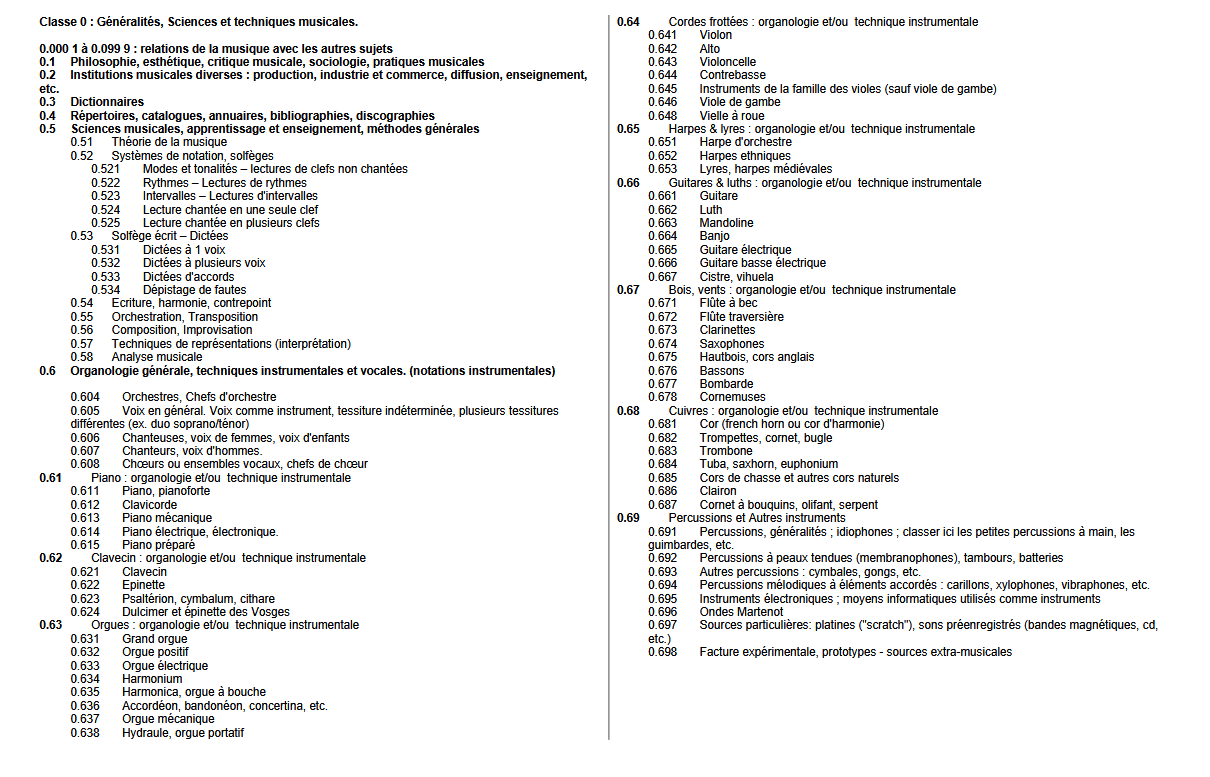
\includegraphics[width=0.6\textwidth]{partie2/images_partie2/images_chapitre4/PCDM4.png}
	\caption{Exemple pour la 1ère classe du Principe de Classement des Documents Musicaux}
\end{figure}

 Par ailleurs, le catalogage des documents musicaux présente des particularités.Lorsque Laurence Karpp-Lahmaidi rédige son mémoire, le modèle FRBR (\textit{Functional Requirements for Bibliographic Records}, ou Spécifications fonctionnelles des notices bibliographiques) n'était pas encore généralisé en France et les documents musicaux faisaient figure de proue dans l'adoption de ce modèle. Le projet ANR Doremus (\textit{Doing Reusable Music Data}), initié en 2014 par la BnF, Radio France et la Philharmonie de Paris a d'ailleurs joué un rôle fondamental dans l'adaptation des modèles de données FRBR/LRM aux spécificités de la musique. En reliant les oeuvres avec leurs interprétations et leurs enregistrements, donnant lieu à des manifestations physiques et numériques, Doremus permet de dépasser les limites des catalogues généralistes non adaptés à la musique et ses complexités (notamment au niveau des transcriptions, enregistrements...). Aujourd'hui, le modèle FRBR a été refondé et a évolué depuis 2017 vers le modèle orienté entité IFLA-LRM (\textit{ International Federation of Library Associations and Institutions - Library Reference Model}). Cela a permis de corriger certaines limites de FRBR, particulièrement problématiques pour la musique. 

Si les fonds patrimoniaux spécialisés en musique font l'objet d'un traitement particulier, mobilisant un réseau d'experts, les sections musique des bibliothèques requièrent également une attention particulière après le bouleversement de la dématérialisation des supports qui les a pleinement touchées. 
A l'heure des plateformes de streaming musical, la bibliothèque fait face à un bouleversement majeur au niveau de ses collections musicales : le nombre d'emprunts de CD chute drastiquement. Sans approfondir quantitativement ce phénomène, analysé par l'élève-conservateur Amandine Pluchet, dans son mémoire de 2012\footnote{Pluchet (Amandine), Les évolutions des sections musique des bibliothèques municipales depuis l’arrivée d’internet, mém. d'étude de conservateur des bibliothèques, dir. X. Galaup, Villeurbanne, Enssib, 2013, 99 p., dactyl. [en ligne], [réf. du 19 juin 2026].} et par Mélanie Lecouteux\footnote{Lecouteux (Mélanie), Nouvelles pratiques professionnelles en section musique, mém. d'étude, dir. C. Paganelli, Montpellier, Université Paul Valéry, 2022. 110 pages.}, nous donnerons ici simplement les grandes tendances des nouvelles pratiques en section musique en bibliothèques. \\

A la suite de la dématérialisation des pratiques musicales, la politique d'acquisition des bibliothèques évolue. Ces dernières doivent proposer une \enquote{offre de collections hybride}(Amandine Pluchet). Même si le modèle de la discothèque de prêt, en vogue dans les années 1960 s'essoufle, il est important de garder une collection physique aux côtés de ressources numériques. 
En effet, le constat d'Amandine Pluchet dans son mémoire est parlant : 
\begin{quotation}
	{A l’heure d’internet et de la musique en ligne, il est plus que
	jamais inconcevable de limiter l’espace musique d’une médiathèque à la seule
	dimension d’une discothèque de prêt. La musique doit s’exprimer dans sa
	diversité, au cœur d’un ensemble de supports aussi bien sonores qu’imprimés:
	CDs et autres enregistrements numériques, mais aussi monographies, et
	périodiques sans oublier les supports destinés aux pratiques amateurs, tels que	partitions et méthodes
	}
\end{quotation}
 Cette politique doit s'effectuer au niveau de l'acquisition, d'une part, qui représente la diversité des supports d'écoute, au moyen d'abonnements à des ressources numériques et d'une veille sur les supports patrimoniaux tels que les vinyles (qui suscitent l'engouement des usagers) et d'autre part au niveau de la médiation musicale. En effet, la politique documentaire ne se limite pas aux acquisitions. Les documents musicaux méritent de faire l'objet d'une programmation culturelle active. 
Par exemple, la bibliothèque patrimoniale  de Dijon, qui conserve un manuscrit musical médiéval, a organisé le 23 avril 2026 un atelier de recherche en partenariat avec l'université de Lausanne et la Haute-Ecole de Musique de Genève. Sur le thème \enquote{Voir, lire, écouter le chansonnier de Dijon}, le public a pu profiter d'un  atelier de recherche suivi d'une visite guidée de la bibliothèque avec une présentation du manuscrit puis d'un concert donné par les étudiants de la HEM. 
En section musique de bibliothèque, les dispositifs de médiation peuvent prendre la forme de borne d'écoute, d'équipements en MAO (Musique Assistée par Ordinateur) avec atelier d'initiation à la prise en main\footnote{Voir à ce sujet le mémoire d'Amandine Pluchet : Pluchet (Amandine),\textit{Les évolutions des sections musique des bibliothèques municipales depuis l’arrivée d’internet}, mém. d'étude de conservateur des bibliothèques, dir. X. Galaup, Villeurbanne, Enssib, 2013, 99 p., dactyl. [en ligne], [réf. du 19 juin 2026], page 61}, ou encore de sélections \enquote{coups de coeur} associées à des concerts dans la bibliothèque. 



\subsection*{Un exemple de charte des collections, la charte des ressources de LaDocumenta.eu}
\label{subsection:Un exemple de charte des collections, la charte des ressources de LaDocumenta.eu}

Appliquées aux bibliothèques d’orchestre, bibliothèques singulières parmi les bibliothèques musicales, ces contraintes d’acquisition et de traitement des collections musicales gagnent à être encadrées par des outils régissant la politique documentaire spécialisée d’une telle bibliothèque.  
Dans le cadre de l'amélioration de la plateforme LaDocumenta.eu, c'est-à-dire la construction de sa nouvelle version (V2) opérée par l'entreprise Reveality.io, il s'est avéré indispensable de réfléchir à l'élaboration d'une \enquote{charte des ressources} de la plateforme. Cet exercice résulte en réalité d'une demande de livrable que le consortium LaDocumenta se doit de fournir au fonds européen qui la soutient, à savoir le programme Europe Creative. C'est dans cet objectif que j'ai été amenée à produire, lors de mon alternance à la bibliothèque de l'orchestre \textit{Insula Orchestra} en tant que chargée de mission LaDocumenta, un pré-livrable\footnote{Ce livrable est consultable dans le volume d'annexes de ce mémoire, sous le titre : Livrable 1 : Charte des ressources de LaDocumenta.eu, pages 4 à 14.} prenant la forme d'une charte des collections. 
Ce livrable se situe donc au coeur de la politique documentaire de la plateforme LaDocumenta.eu. \\
Comme nous l'avons vu, la charte des collections est l'un des outils clés de la politique documentaire.
\begin{quotation}
La charte des collections définit la politique documentaire générale de l’établissement. Elle présente l’organisation de la bibliothèque et en définit les objectifs généraux (supports, secteurs documentaires, critères de choix ou d’exclusion, règles d’élimination ou de conservation, traitement des suggestions ou des dons, etc.). C’est un document interne, porté par la direction et obligatoirement validé par la tutelle, mais qui peut aussi être communiqué au public. C’est un outil destiné à durer plusieurs années, qui doit donc être ré-évalué régulièrement\footnote{Définition issue du groupe Poldoc de l'Association des bibliothécaires de France (ABF):\url{https://www.poldoc.abf.asso.fr/boite-a-outils/}.}.
\end{quotation}

Elle régit les pratiques \enquote{des secteurs documentaires, les supports, les critères de choix et d'exclusion, les règles d'élimination et de conservation ainsi que le traitement des suggestions des adhérents, des dons et des échanges\footnote{Henard (Charlotte), \textit{La politique documentaire, de quoi parle-t-on et comment faire ?}, support de cours de l'ABF, Toulouse, Médiad'Oc, 2024-2025.}}.
La particularité de la charte des collections de LaDocumenta.eu consiste en la matérialité numérique de cette bibliothèque. C'est pour cette raison qu'il a été décidé d'appeler ce document une \enquote{charte des ressources}, en référence aux ressources numériques qui la composent. 

Sur les conseils de la directrice de la bibliothèque de l'Ecole Nationale des Chartes, Camille Degez-Selves, j'ai pris connaissance de la charte documentaire de l'ENSSIB, validée en février 2026 et publiée en avril, qui a été reprise pour construire le plan de la charte des ressources de LaDocumenta.eu\footnote{Pour voir la charte des ressources de LaDocumenta.eu, consulter le volume d'annexes portant sur les livrables technique de ce mémoire, il s'agit du 1er livrable, intitulé \enquote{Charte des ressources de LaDocumenta.eu}, page 5}.
En me référant à la charte documentaire de l'ENSSIB (Ecole Nationale Supérieure des Sciences de l'Information et des Bibliothèques)\footnote{Voir la charte documentaire 2026 de l'ENSSIB à cette adresse : \url{https://www.enssib.fr/sites/enssib.fr/files/inline-files/Charte-documentaire-Enssib-2026.pdf}}, j'ai choisi d'élaborer la charte des collections de LaDocumenta.eu en suivant ce plan : 
\begin{figure}[H]
	\centering
	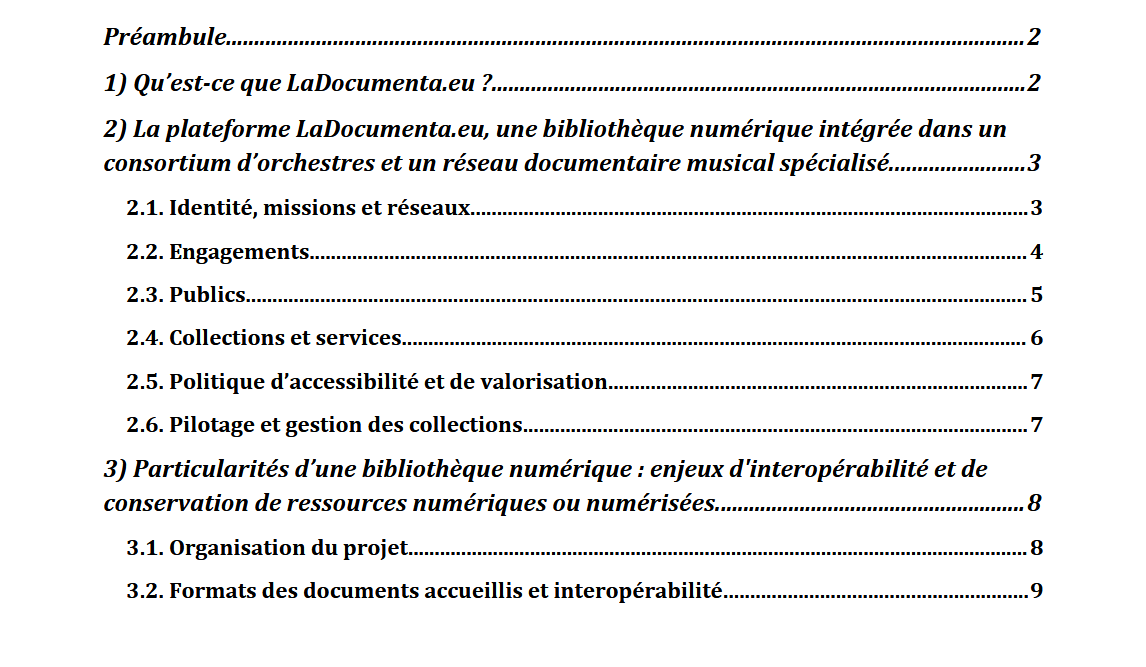
\includegraphics[width=0.9\textwidth]{partie2/images_partie2/images_chapitre4/plan_charte_ressources.png}
	\caption{Capture d'écran du plan du pré-livrable de charte des ressources de LaDocumenta.eu}
\end{figure}

Il a été bénéfique de réutiliser les grandes idées de la charte documentaire de l'ENSSIB pour l'adapter au cas de LaDocumenta.eu. 

\begin{itemize}
	\item Le \textbf{préambule} a permis d'introduire aux futurs lecteurs l'enjeu d'une charte documentaire. Il permet d'affirmer l'utilité du document tout en en précisant l'utilisation et les conditions de publication (comme la validation préalable du conseil scientifique du consortium)
	\item La \textbf{première partie} a permis de présenter clairement les objectifs de LaDocumenta.eu, à la fois consortium et plateforme, base de données et bibliothèque numérique, site internet du consortium et interface privée des membres du consortium, en remplacement d'un éventuel Système de Gestion de Bibliothèque (SIGB) comme ceux des logiciels PMB. 
	Cette partie présente également les enjeux de la plateforme, qui seront détaillés ensuite. 
	\item La \textbf{deuxième partie} explicite la différence entre une politique documentaire généraliste et une politique doublement spécialisée comme celle de LaDocumenta.eu, avec d'une part la spécialité musicale, et d'autre part le support numérique.
	
	\begin{itemize}
		\item Le premier point s'appuie sur un entretien mené avec l'équipe de développeurs de la plateforme : l'entreprise Reveality.io\footnote{Entretien avec Maxime Touroute, développeur de LaDocumenta.eu, mené le 1er juillet 2026, avec contributions écrites de Marc Karassev, également développeur de LaDocumenta.eu. La grille d'entretien est consultable en annexes.} pour avoir un socle de connaissances solide sur les précisions techniques de la plateforme. L'objectif est d'expliquer simplement le fonctionnement de la plateforme. 
		Il concerne également les missions et aspirations futures de la plateforme.
		
		\item Le deuxième point porte sur les engagements de la plateforme. L'idée de ce développement est de s'inscrire dans le réseau européen Europe creative, pour lequel LaDocumenta.eu a été lauréate et d'affirmer les convictions du consortium, dans une continuité avec les priorités européennes des campagnes de financement. 
		
		\item Le troisième point présente les publics de la plateforme en les regroupant dans des catégories. Ces catégories ont été réutilisées ensuite pour élaborer le 3e livrable\footnote{Voir à ce propos le 3e livrable du volume des annexes techniques : \enquote{Usages de la Documenta.eu et scénario d'utilisation de l'IA} de ce mémoire, portant sur les usages IA de la plateforme.} 
		
		\item Le quatrième point constitue le coeur de la charte documentaire de LaDocumenta.eu puisqu'il informe le lecteur sur le corpus de la plateforme. Dans ce point est expliqué l'organisation même des ressources de la plateforme, suivant le découpage des phases d'une production musicale (pré-production, production, concert et post-production\footnote{Ce découpage en phases de production, au sujet de l'organisation des ressources, est l'oeuvre de Kai Kopp, directeur du comité scientifique du consortium}).
		\item Le cinquième point concerne l'accessibilité et la valorisation des collections. Après avoir rappelé l'accessibilité, fidèle principe d'ouverture des bibliothèques. Cette section précise les modalités d'accès, nécessairement adaptées en raison du caractère numérique de la plateforme.\\ 
		Il y a deux points d'attention dans cette section : la consultation et le téléchargement des ressources ainsi que la gestion des ressources sous droits.\\
	Ce dernier point, grisé, n'a pas pu être traité à cet état d'avancement de ce pré-livrable. En effet, ce questionnement convoque des considérations de droit de la propriété intellectuelle qui seront abordées en conseil scientifique prochainement et qui n'avaient pas été tranchées ni lors de l'élaboration de ce livrable, ni à mon départ de stage. Il semblerait par ailleurs que cette question devrait faire l'objet d'une réflexion à part entière dans les projets de financement suivants. Un profil de doctorant en droit de la propriété intellectuelle, travaillant sur les questions de droit en contexte numérique, a été évoqué par l'IreMus, partenaire scientifique de la plateforme. \\
	J'ai toutefois proposé une ébauche de réflexion dans le livrable et indiqué des références bibliographiques à mes responsables. Ensemble, nous avons convenu que ces considérations juridiques poseraient majoritairement problème quant à la communicabilité des ressources. Nous pouvons donc dès à présent envisager les questionnements qui seront à l'ordre du jour des réflexions du comité scientifique, notamment en regard des implications UX de la plateforme en présence d'un document sous droits. Nous pouvons donc supposer que, comme dans Gallica, une ressource sous droits pourrait ne pas apparaître sur la plateforme utilisateur mais seulement sur la plateforme de l'orchestre contributeur. L'usager intéressé pourrait être invité à consulter en présentiel la ressource à la bibliothèque de l'ensemble contributeur, sur un intranet et sans moyen de télécharger la ressource. L'usager pourrait également se voir proposer un fichier filigrané rendant impossible la lecture de la ressource complète, lui permettant toutefois de pouvoir prendre connaissance de l'incipit de la ressource par exemple. 
		\item Le sixième point porte sur le pilotage et la gestion des collections. Il est constitué de trois thématiques que sont : l'administration de la plateforme, la collecte et le dépôt des ressources de la plateforme ainsi que la conservation des ressources de la plateforme. Pour ce sixième point, lui aussi grisé, il ne m'a pas été possible non plus de proposer un texte car les critères d'admission d'une plateforme, les modalités de collecte ainsi que la politique de pilotage des collections n'avaient pas encore fait l'objet de directives de la part du comité scientifique. Comme pour les questions juridiques, j'ai indiqué les principales thématiques qui devraient être abordées prochainement, comme les critères de sélection des ressources (qualité, rareté...), la politique en cas de doublon, ou encore les enjeux de pérennité des collections numériques mais il était impossible à ce stade de proposer une réflexion de mon côté, sans concertation avec le comité scientifique. 
	\end{itemize}
\item La \textbf{troisième partie} sera détaillée dans le chapitre suivant car elle porte davantage sur les enjeux numériques de standardisation et d'intéropérabilité que sur l'élaboration d'une charte des collections. La problématique des référentiels, non abordée dans ce chapitre illustre en effet les questionnements que pose la plateforme au sujet de la standardisation des données et de l'intéropérabilité.  Après avoir détaillé la politique documentaire de la plateforme LaDocumenta.eu dans ce quatrième chapitre, l'on s'attelera à présenter les enjeux de la standardisation des données des plateformes numériques dans un objectif de construire l'intéropérabilité des données musicales. 	
\end{itemize}	
